\chapter{Background and Preliminaries}\label{ch:problem}
%---------------------------------------------------------

\section{Classical Feedback vs Adaptive Control}
Control of a system can be broken into two required elements.  There is the requirement to control the system from:
\begin{enumerate}
 \item disturbances which affect the controlled states 
 \item disturbances which affect the performance of the system as a whole
\end{enumerate}
Classical feedback control seeks to solve the first type of disturbance.  This form of control is meticulously tuned to achieve the desired overshoot and settling time for example.  The important assumption that is made by classical feedback controllers is that the underlying plant/system performance is not changing.  For example, the cruise control that maintains a vehicle's speed assumes that the available horsepower of the car is fixed.  This is a fairly good assumption as the horsepower with respect to rpm available at sea level and at 5,000 feet for an internal combustion engine is constant enough that a fixed gain feedback controller would perform well at maintaining the speed of the vehicle in both environments.  In the case of an airplane, the dynamic pressure is proportional to velocity squared and can drastically change the performance of the aircraft.  In this case, the constant system performance assumption can cause a fixed gain classical feedback controller to go unstable at higher dynamic pressures (higher airspeeds).   Conversely, adaptive controllers assume that the system performance is unknown and is likely to vary with time.  Adaptive control seeks to ensure a system's performance in terms of characteristics like damping ratio and settling time are kept constant regardless of a plant dynamics that may be unknown and time varying.  For both classical and adaptive control there exists some form of error which drives the controller.  In the case of classical feedback, the error is calculated between the command and the feedback state of the plant. In adaptive control (in general), the error is calculated between the outputs of the desired reference model and real plant's measured performance.

Figure~\ref{fig:why_adaptive_control} outlines the decision making process a controls engineer makes when deciding the type of controller needed for a given circumstance.

%I would not spend too much time here. What critical is to demonstrate the fundamental difference. In the case of classical feedback, the error is calculated between the command and the feedback of the plant. In adaptive control (in general) the error is calculated between the outputs of the reference model and real plant.


\begin{figure}[h!]
 \centering
  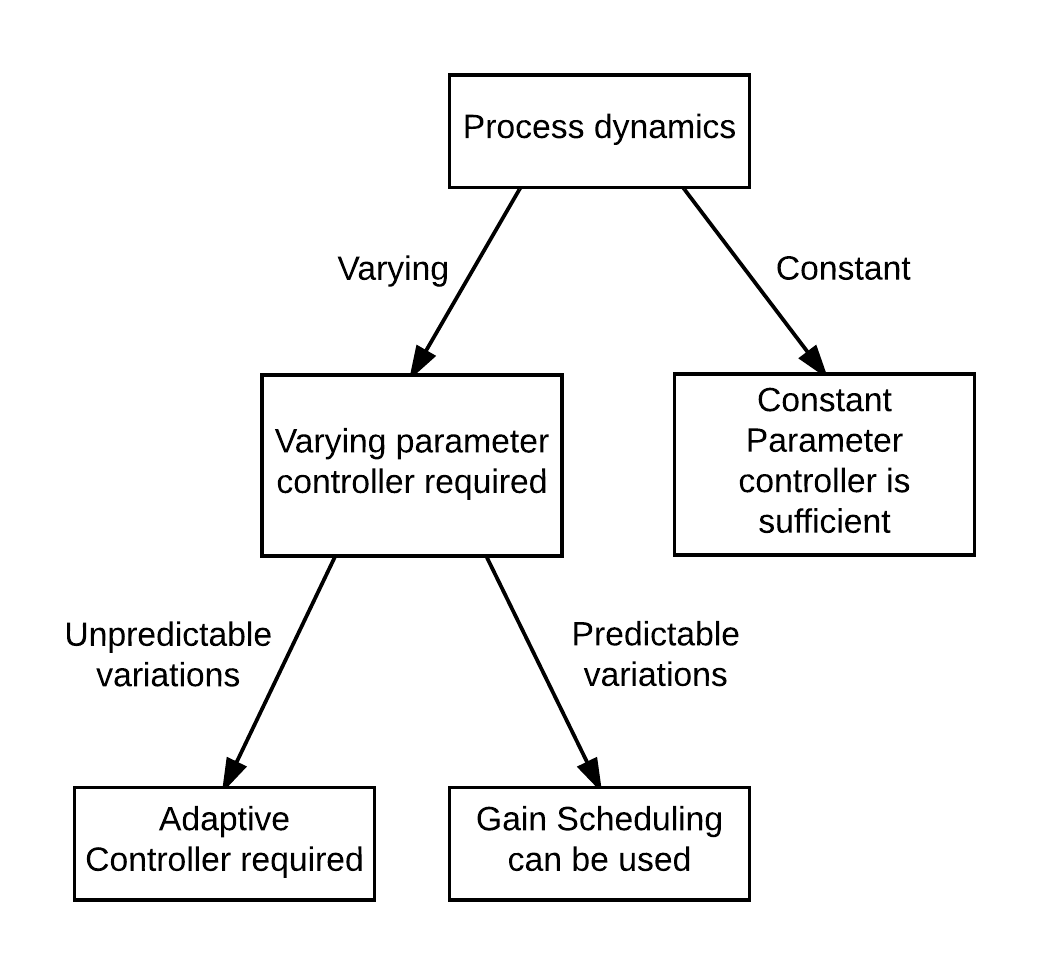
\includegraphics[width=0.5\textwidth]{why_adaptive_control.png}
  \caption{Determine if adaptive control should be used}
  \label{fig:why_adaptive_control}
\end{figure}


%---------------------------------------------------------
\section{Model Reference Adaptive Control}
\ac{MRAC} establishes the foundation for most of modern robust adaptive control.  Its structure is intuitive in nature and seeks to define a system's response to a command signal with a reference model.  Unlike traditional feedback where the error signal is generated with respect to state error, \ac{MRAC} attempts to achieve a system response with respect to some reference model performance. \ac{MRAC} assumes that there is some nominal response of the system which can be characterized with a model of unknown parameters.  The error between the model response and the system response generates the error for an 'adjustment mechanism' to learn the unknown model parameters.

\begin{figure}[h!]
 \centering
  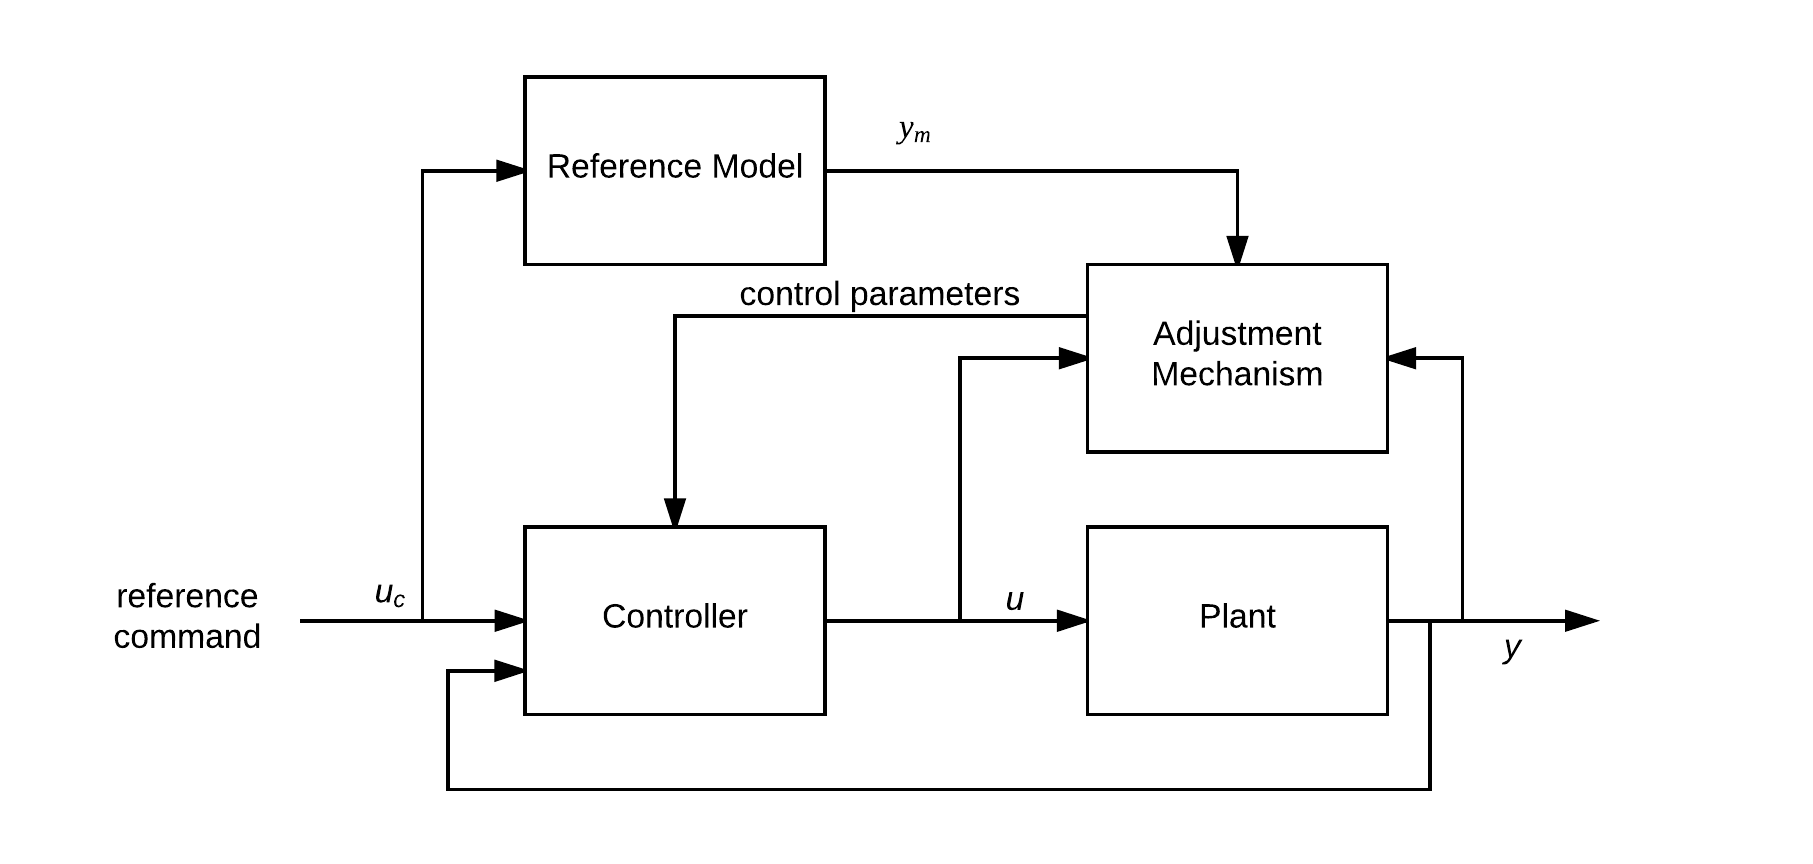
\includegraphics[width=1.0\textwidth]{traditional_MRAC.png}
  \caption{Traditional \ac{MRAC} architecture }
  \label{fig:traditional_mrac}
\end{figure}

Figure~\ref{fig:traditional_mrac} illustrates a topology where a traditional feedback controller is established as an inner loop and the 'Reference Model' and 'Adjustment Mechanism' is established as an outer loop.  The outer loop attempts to minimize the error between the reference model output and the plant output.  Using this error to learn the system parameters can be done utilizing one of two methods; gradient descent or stability theory.

\subsection{MIT Rule - Gradient Decent}
One of the first approaches to \ac{MRAC} controllers was implemented at the Instrument Labs at MIT (now known as Draper Labs).  The gradient descent based method was called the 'MIT Rule' for this reason \cite{aastrom2013adaptive}.  This method attempts to learn some unknown parameter by descending the gradient of the error between the reference model and the plant output.

Given the simple first order system $G(s)$:
\begin{equation}
G(s) = k_{dc}\frac{1}{s+1}
\end{equation}

where $k_{dc}$ is some unknown feedforward gain.  In the case of the MIT rule, $k_{dc}$ is the parameter to be learned and is defined as $\theta$.  The first step in the MIT rule is to establish a cost (or loss) function.  One example of a cost function $J(\theta)$ is:
\begin{equation}
J(\theta) = \frac{1}{2}e^2
\end{equation}
\begin{equation}
e=y-y_m
\end{equation}

where $e$ is error, $y$ is the plant output, and $y_m$ is the model output.

In order for the cost function to be minimized, the negative gradient of the cost function is calculated and used to correct the a priori estimate.  This method takes the following form where $\gamma$ is the adaptation gain:
\begin{equation}
\frac{d\theta}{dt}=-\gamma \frac{\partial{J}}{\partial{\theta}} =-\gamma e\frac{\partial{e}}{\partial{\theta}}
\end{equation}

The stability of this method is very system dependent and heavily relies on trial and error to ensure the adaptation gain $(\gamma)$ is not too high.  This usually requires low adaptation rates for most systems and may not produce adequate results.  It should also be noted that this method presupposes there is adequate persistence of excitation.  Without a frequency rich error signal being generated by adequate persistence of excitation, the model will fail to adapt.  This method also offers no guarantees that the learned parameters are actually the correct values.

\subsection{Lyapunov Stability Criteria}

Aerospace controllers tend to use linear controllers for their simplicity and well-understood robustness characteristics.  This is despite the fact that the applications of these linear controllers are applied to a non-linear dynamical system such as attitude control with varying dynamic pressure.  Adaptive Controllers are non-linear and may offer performance benefits to non-linear systems as seen in aforementioned aerospace applications.  However, non-linear controller's robustness properties need to be evaluated.  The Lyapunov stability criteria offer methods of evaluating these controller's boundedness and robustness behavior.

Aleksandr Lyapunov was a Russian mathematician who's work was published in 1892 \cite{lyapunov1892general} concerning the behavior of non-linear systems close to equilibrium without having to rigorously find the unique solutions to difficult differential equations used to model the system.  His work was largely overlooked until the Cold War when aerospace solutions required a more rigorous approach to analyzing non-linear control robustness.  Modern non-linear control engineers extensively utilize Lyapunov's techniques to design and evaluate non-linear controllers.

\subsubsection{Lyapunov Stability Definitions}

Lyapunov's methods attempt to evaluate autonomous nonlinear dynamical systems within the bounds of three classifications.  In this case, the autonomous system is defined as definable set of ordinary differential equations which are not explicitly dependent upon the independent variable.  These classifications can be used to define a nonlinear system as Lyapunov stable, asymptotically stable, or exponentially stable.

Given the following autonomous nonlinear dynamical system:

 \begin{equation}
\dot{x}(t)=f(x(t)), \qquad x(0)=x_0
\end{equation}

where $f$ has equilibrium at $x_e$ :
 \begin{equation}
f(x_e) = 0
\end{equation}

then the equilibrium is said to be:
\begin{enumerate}
 \item \textbf{Lyapunov Stable} \newline
 for every $\epsilon > 0$ there exists a $\delta > 0$ such that, if \: $\norm{x(0) - x_e} < \delta$, then for every $t \geq 0$ we have  $ \norm{x(t) - x_e} < \epsilon$ 
 \item \textbf{Asymptotically Stable} \newline
 if the system is Lyapunov stable and there exists a $\delta > 0$ such that if \: $\norm{x(0) - x_e}  < \delta$, then $\displaystyle \lim_{t\to \infty} \norm{x(t)-x_e} =0$
 \item \textbf{Exponentially Stable} \newline
 if the system is asymptotically stable and there exists $\alpha > 0, \beta > 0, \delta > 0$ such that if $\norm{x(0)-x_e}<\delta$, then \:$\norm{x(t)-x_e} \leq \alpha \norm{x(0)-x_e} e^{-\beta t}$, for all $t \geq 0$
\end{enumerate}

Being Lyapunov stable infers that if a system is near equilibrium then it will indefinitely remain near equilibrium.  If the system if found to be asymptotically stable then it eventually will achieve equilibrium as $t\to \infty$ and being exponentially stable implies it reaches equilibrium even faster.

\subsubsection{Lyapunov's Second Method}
 
Lyapunov's second proposed method is also known as Lyapunov stability criteria.  This method offers a less tenuous method for evaluating mathematically non-ideal systems.  Lyapunov analysis of the linearized system around equilibrium can be cumbersome in the case where equilibrium is at the origin or the eigenvalues are purely imaginary.  In this case, the solutions can rapidly depart to infinity or approach zero with little perturbation to the eigenvalues.  Lyapunov's second method offers an alternative approach for classifying a system's stability using a concept that is similar to how energy is defined in classical dynamics.

Conceptually, Lyapunov's second method can be compared to evaluating the energy of a vibrating spring mass system.  The energy of the unforced spring mass system will dissipate energy due to friction and or damping etc.  This trend of energy leaving the system towards some 'attractor' is evidence of the system's stability characteristics and identifies that there will be some stable end state.  Likewise, Lyapunov's second method characterizes this with the use of a Lyapunov candidate function $V(x)$.  It is important to note that Lyapunov realized that the candidate function can be any function so as long as one candidate function is found in agreement with the stability criteria.  It is then said to be Lyapunov stable if any candidate equation is found and meets the stability criteria.  This means that it is only incumbent upon the engineer to find one candidate equation to meet the criteria.  This can be an iterative process of trying multiple energy like equations.  A common approach is to model the Lyapunov candidate equation as kinetic energy $(\frac{1}{2}u^2)$.  Lyapunov realized that characterizing the energy of a nonlinear system could be almost impossible for some cases, but this approach could prove stability without the rigorous knowledge of the true system's energy.

Lyapunov's second method defines a system as Lyapunov Stable for a system $\dot{x}=f(x)$ having an equilibrium point at $x=0$ where the Lyapunov candidate function $V(x):\mathbb{R}^n \rightarrow \mathbb{R}$ such that:
\begin{itemize}
 \item $V(x)=0$ if and only if $x=0$
 \item $V(x)>0$ if and only if $x\neq0$
 \item $\dot{V}(x)=\frac{d}{dt}V(x)=\sum\limits_{i=1}^{n} \frac{\partial V}{\partial x_i}f_i(x) \leq 0$, for all values of $x\neq 0$  
\end{itemize}

if $\dot{V}(x) < 0$ for $x\neq 0$ then system is asymptotically stable.

To determine if the system is globally stable, it is additionally required to prove the condition of radial unboundedness.















